\section{Recurrent Neural Networks}
\label{sec:recurrent_neural_networks}

The two major types of neural networks are distinguished by the structure of
their internal weights.  Feedforward networks simply pipe their input through
all the layers towards the output. They have proven very useful for tasks that
require static, non-linear input-output mappings such as pattern recognition or
classification.  Processing time series is a different task because, to model a
sequence, the network needs information about the past. In a FNN this is not
the case.  An input vector $\vt{u}$ that is fed into the network $F$ does not
contain information about previous or future inputs and the prediction $\vt{y}$
has to be made solely based on the current input:
\begin{equation}
  \vt{y} = F(\vt{u})
\end{equation}

\begin{figure}
  \begin{minipage}[b]{.4\textwidth}
    \centering
    \FeedForwardNet{1}
    Feedforward Network
  \end{minipage}
  \hspace{.05\textwidth}
  \begin{minipage}[b]{.5\textwidth}
    \centering
    \RecurrentNet
    Recurrent Network
  \end{minipage}
  \caption{The traditional feedforward network on the left only exhibits
  forward connections while the recurrent network on the right has cyclic
  connections within or possibly even between layers if there is more than one
  hidden weight matrix.}
  \label{fig:fnn_rnn}
\end{figure}

In contrast, recurrent neural networks (RNN) possess cyclic weight connections.
The outputs of a layer have feedback weights that are connected to the same or
a previous layer.  This cyclic nature of RNNs mathematically makes them
dynamical systems [\cite{FUNAHASHI}] and it can be shown that they are
\emph{Turing complete} [\cite{siegelmann1991}]. A brief description on the analogies
between RNNs and dynamical systems is given in
Sec.~\ref{ssub:state_space_model}. Roughly, RNNs maintain an internal state
$\vt{x}$ at all times which acts as a memory of previous inputs. At every time
step the network receives the previous internal state along with an input
vector and returns a prediction $\vt{y}$ as well as an updated internal state
$\vt{x}$:
\begin{equation}
  \label{eq:recurrent_network_F}
  \vt{y}, \text{ } \vt{x} = F(\vt{u}, \vec{x}_{t-1}).
\end{equation}

This enables RNNs to process time series data and they are thus qualified for
tasks such as filtering, dynamic pattern recognition, and prediction.  RNNs are
most widely used in speech recognition or other language processing tasks, but
they are also highly interesting from a neurological point of view, as all
biological neural networks are recurrent.  Generally, they are highly promising
tools for non-linear time series modelling.  They can be run in a
self-monitoring fashion, which makes them very interesting for an automated
outlier detection in large scale time series data.  Especially in the field of
Natural Language Processing (NLP), RNNs have achieved impressive results while
requiring little preprocessing of datasets [\cite{sutskever2011generating}].


\subsection{State Space Model}
\label{ssub:state_space_model}

The simplest dynamical system in discrete time is defined by a state space $M$,
a set of times $T$, and an evolution function $\Phi$.  The function $\Phi$ maps
a given state $\vec{x}_{t-1} \in M$ at time $t \in T$ to a new state $\vt{x}$:
\begin{equation}
  \vt{x} = \Phi(\vec{x}_{t-1}).
\end{equation}

A dynamical system with inputs $\vt{u}$ and outputs $\vt{y}$ is defined by
the state space representation:
\begin{align}
  \vt{x} &= \Phi(\vt{u}, \vec{x}_{t-1}), \\
  \vt{y} &= \Psi(\vt{u}, \vec{x}_{t-1}).
\end{align}

In a basic RNN the two functions $\Phi$ and $\Psi$ are defined with an input
matrix $\wmatr{in}$, a recurrent weight matrix $\wmatr{}$, and an output matrix
$\wmatr{out}$:
\begin{align}
  \label{eq:state_space}
  \vt{x} &= \varphi(\wmatr{in} \vt{u} + \wmatr{}\vec{x}_{t-1}), \\
  \label{eq:readout}
  \vt{y} &= \psi(\wmatr{out} \vt{x}),
\end{align}

where $\varphi$ denotes the component-wise applied, non-linear, state
activation function. In RNNs a typical choice is the hyperbolic tangent.  The
output activation function $\psi$ is commonly chosen to be the identity
function, resulting in a linear output layer.  A flow chart of the basic RNN is
shown in Fig.~\ref{fig:rnn_flow_chart}.  The input weights $\wmatr{in}$ have
dimensions $n \times m$, hidden weights $\wmatr{}$: $n \times n$ and
output weights $\wmatr{out}$: $n \times k$. In the simple RNN the input is
not utilized by the output layer, but would be entirely possible to introduce
another matrix to do this.

An input series $\mathbf{u}$ of length $N$ that is fed to the network one by
one produces $N$ internal states.

\begin{equation}
  \mathbf{x} = (\vt{x}, \vec{x}_{t+1}, ..., \vec{x}_{t+N}),
\end{equation}
\begin{figure}
  \centering
  \RNNFlowChart
  \caption{Basic RNN cell flow chart. The recurrent weights are enclosed by the
  non-linearity $\varphi$, the output weights by the function $\psi$.}
  \label{fig:rnn_flow_chart}
\end{figure}



From Eq.~\ref{eq:state_space}, it becomes evident that the internal state acts
as a kind of memory of the network.  This memory is dynamic as opposed to the
static memory brought about by weight adjustments of GD.  The latter is called
long-term memory. The dynamic memory of the internal RNN state is termed
\emph{short-term memory} (STM). STM will be further discussed in
Sec.~\ref{sub:short_term_memory}  and brief computational analysis of the STM
capacity is given in Sec.~\ref{sec:short_term_memory}. 

Every new input overwrites a part of the previous internal state, gradually
encoding the input sequence into $\vt{x}$.  The length of an input sequence
that can be encoded into $\vt{x}$ depends on the size of the internal state and
on the two matrices $\wmatr{in}$ and $\wmatr{}$.  Generally, the state size $n$
must be much larger than the input size $m$, in order to create an effective
RNN. How an RNN is trained in the light of a time dependency of the weights is
described in Sec.~\ref{sub:training_recurrent_neural_networks}.

As the internal states now contain information both about current and past
inputs, it is possible for the output matrix $\wmatr{out}$ to create an educated
prediction of the next frame.  An RNN that receives its output as the next
input is called a freely running RNN and enables predictions further into the
future as depicted in Fig.~\ref{fig:annotated_rnn}.  Of course, in this case the
number of input and output units must be the same: $k = m$.

\begin{figure}
  \centering
  \RecurrentNetAnnotated
  \caption{RNN setup that is able to predict $n$ steps into the future by
    feeding the output back into the input. The input and output layers are
    fully connected. The internal weight connections can be sparse to speed
    up the network for large reservoir sizes.
  }
  \label{fig:annotated_rnn}
\end{figure}



\subsection{Training Recurrent Neural Networks}
\label{sub:training_recurrent_neural_networks}

There exist various different methods of training recurrent networks, which all
have their own benefits and drawbacks or just perform better or worse at
different tasks. No clear favourable approach, like the mini-batch GD algorithm
for feedfoward networks, was found yet.  This is due to several obstacles that
arise specifically during RNN training, which will be discussed below.  The
three most common methods are \emph{Backpropagation Through Time} (BPTT),
\emph{Real-time Recurrent Learning} (RTRL, [\cite{williams1989}]), and
\emph{Extended Kalman Filtering} (EKF, [\cite{williams1992}]), the first of which
will be treated below.

\subsubsection{Backpropagation Through Time}
\label{ssub:backpropagation_through_time}

BPTT is an adapted form the of classic backpropagation algorithm of feedforward
networks as described in Sec.~\ref{sec:feedforward_neural_networks} and was
developed for the first time by~[\cite{mozerBPTT}].  The
cyclic connections of RNNs prevent the direct application of the
backpropagation algorithm.  One solution is to \emph{unroll} the network in
time by stacking the network on top of itself for a certain number of time
steps.  The depth of unrolling is determined by the length $N$ of the sequence
$\mathbf{u}$ that is fed into the network.

By unrolling the network in time, one practically ends up with a very deep
feedforward network with shared weights between the stacked layers of clones of
the network.  In the forward pass each clone, which now corresponds to a time
step in the sequence, receives the corresponding input $\vt{u}$ and updates its
own internal state $\vt{x}$.  The internal state of each clone depends on its
input and on the internal state of the previous layer (at time $t-1$).  Finally
the output $\vt{y}$ is computed by each clone.  The loss function that is
minimized is defined by:
\begin{equation}
  \mathcal{L} = \sum_{t=0}^{N} \mathcal{L}_t
              = \sum_{t=0}^{N} || \vt{d} - \vt{y} ||_2.
\end{equation}

The weight adjustment is now done by a typical gradient descent algorithm.  By
collecting all the weights and biases of the state space model in the variable
$\Theta$ we can write the weight adjustment as:
\begin{equation}
  \label{eq:batch_update}
  \Theta' = \Theta + \eta \sum_t \frac{\partial \mathcal{L}_t}{\partial \Theta}
\end{equation}

The expression for the gradient of the cost can by derived by applying the
chain rule:
\begin{equation}
  \newcommand{\loss}{\mathcal{L}_t}
  \dd{\loss}{\Theta} = \dd{\loss}{\vt{x}} \dd{\vt{x}}{\Theta}
  = \dd{\loss}{\vt{x}} \dd{\vt{x}}{\vec{x}_{t-1}} \dd{\vec{x}_{t-1}}{\Theta},
\end{equation}

which results in a product of derivatives, as every state depends on the
previous one.
\begin{align}
  \newcommand{\loss}{\mathcal{L}_t}
  \dd{\loss}{\Theta} = \dd{\loss}{\vt{x}} \dd{\vt{x}}{\vec{x}_{0}} \dd{\vec{x}_{0}}{\Theta} \\
  \dd{\vt{x}}{\vec{x}_{0}} = \prod_{i=1}^t \dd{\vec{x}_i}{\vec{x}_{i-1}} \label{eq:dxtdxN}
\end{align}

The last derivative of the state $\vec{x}_0$ denotes the derivative of the first
state (starting to count from the perspective of the forward pass) of the
unrolled network, which is a constant with respect to $\Theta$.  From
Eq.~\ref{eq:dxtdxN} one can see the origin of the vanishing and exploding
gradient problems.  If the individual derivatives $\dd{\vt{x}}{\vec{x}_{0}}$ are
small, the gradient, being product of these derivatives, vanishes very quickly
and explodes if they are large.  It can be shown that it `[...] is
\textit{sufficient} for the largest eigenvalue $\lambda_1$ of the recurrent
weight matrix to be smaller than one for long term components to vanish (as $t
\rightarrow \infty$) and \textit{necessary} for  it  to  be  larger  than  one
for  gradients  to explode.' -- [\cite{razvan2012}].
By bounding the spectral radius
of the recurrent weights to be smaller than one, it is thus possible to avoid
the exploding gradient problem. A solution to the vanishing gradient problem is
more complicated and involves advanced network architectures such as the long
short-term memory (LSTM) unit [\cite{lstm}].  It introduces additional input,
forget, and output layers, but the essential part is that one of the recurrent maps of
the unit is the identity function.  The derivatives in Eq.~\ref{eq:dxtdxN}
become one and the gradient can flow through many layers.  A completely
different approach is to avoid training the recurrent weights altogether, which
will be described in Sec.~\ref{sec:reservoir_computing}.


\subsection{The Bifurcating State Space}%
\label{sub:the_bifurcating_state_space}

Another problem that arises with the optimization of recurrent weights is that
the state space is not necessarily continuous, which was shown by
[\cite{doya1992}].  The points at which the state space has discontinuities are
called \emph{bifurcations} and are extensively studied in non-linear dynamics.
They can cause discontinuities in the state space and thus impair the learning
or prevent convergence to a local minimum completely.  To understand what
bifurcations are and how they affect RNN training, we will consider the
recurrent part of a single unit RNN with the hyperbolic tangent as the
activation function.  If the RNN has only one unit the state $\vt{x}$, as well
as the weights and biases become scalars:
\begin{equation}
  \label{eq:single_unit_rnn}
  x_{t+1} = \tanh(w x_t + b).
\end{equation}
The parameter $w$ denotes the scalar weight of the single unit and $b = w_{in}
u_t$ will serve as the bias of a constant input of $u_t = 1$.  In
Fig.~\ref{fig:bif_evolution} we can see the evolution of $x_t$.  Depending on
different initial values $x_0$ and network parameters, the state converges to
different values for $t$ towards infinity. These values are called \emph{fixed
points} $x^*$ and for them $x_t = x_{t+1}$ holds.  In particular, fixed points
that the state converges to are called \emph{stable} fixed points (or
\emph{attractors}).  The second kind of fixed points are \emph{unstable}.  The
slightest deviation from an unstable fixed point will result in a flow away
from the point, which is why they are also called \emph{repellers}.  In the
first three cases of Fig.~\ref{fig:bif_evolution} a fixed point is always
reached. The fourth example in the lower right shows representatives of
the oscillating fixed point, more specifically \emph{period-2 cycles}, that
repeat every second iteration.
\begin{figure}
  \centering
  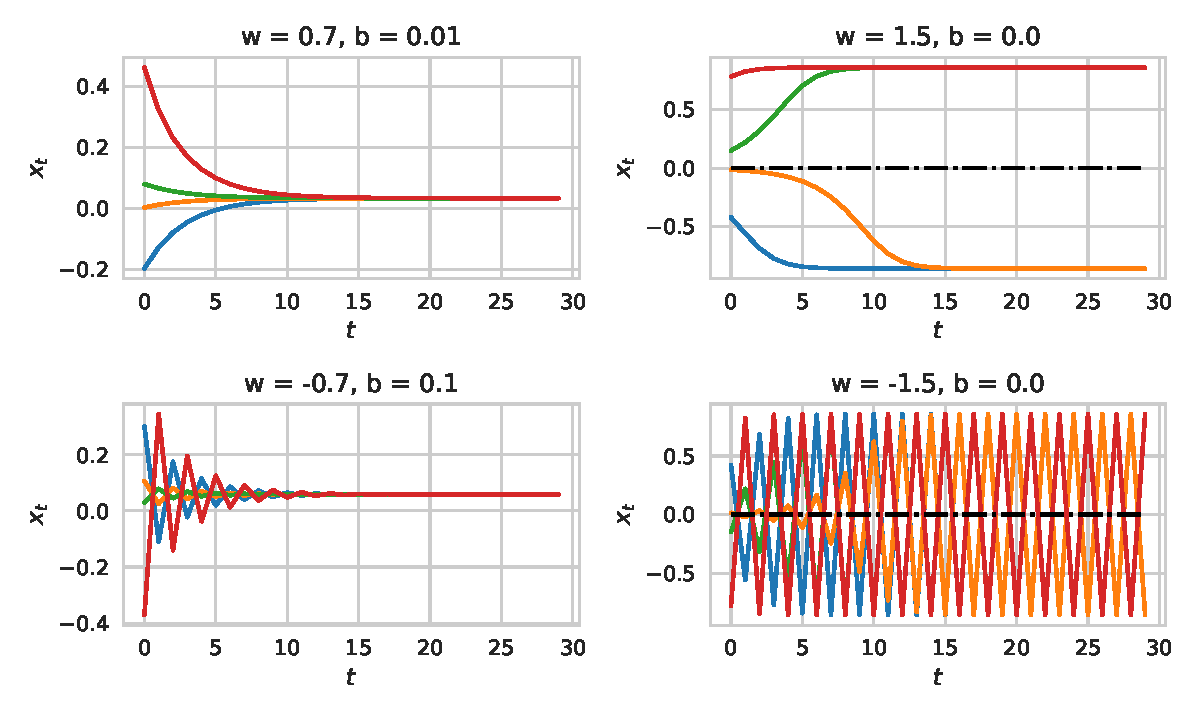
\includegraphics[width=\linewidth]{bif_evolution.pdf}
  \caption{Evolution of $x_t$ over time for different parameters $w$ and $b$.
    Dashed lines show unstable fixed points. Apart from the expected fixed points
    that $x_t$ converges to over time, there are also oscillations visible in
    the last plot. Such oscillations that repeat every 2 iterations are called
    \emph{period-2 cycles} and they appear when $w<-1$.}
  \label{fig:bif_evolution}
\end{figure}
\begin{figure}
  \centering
  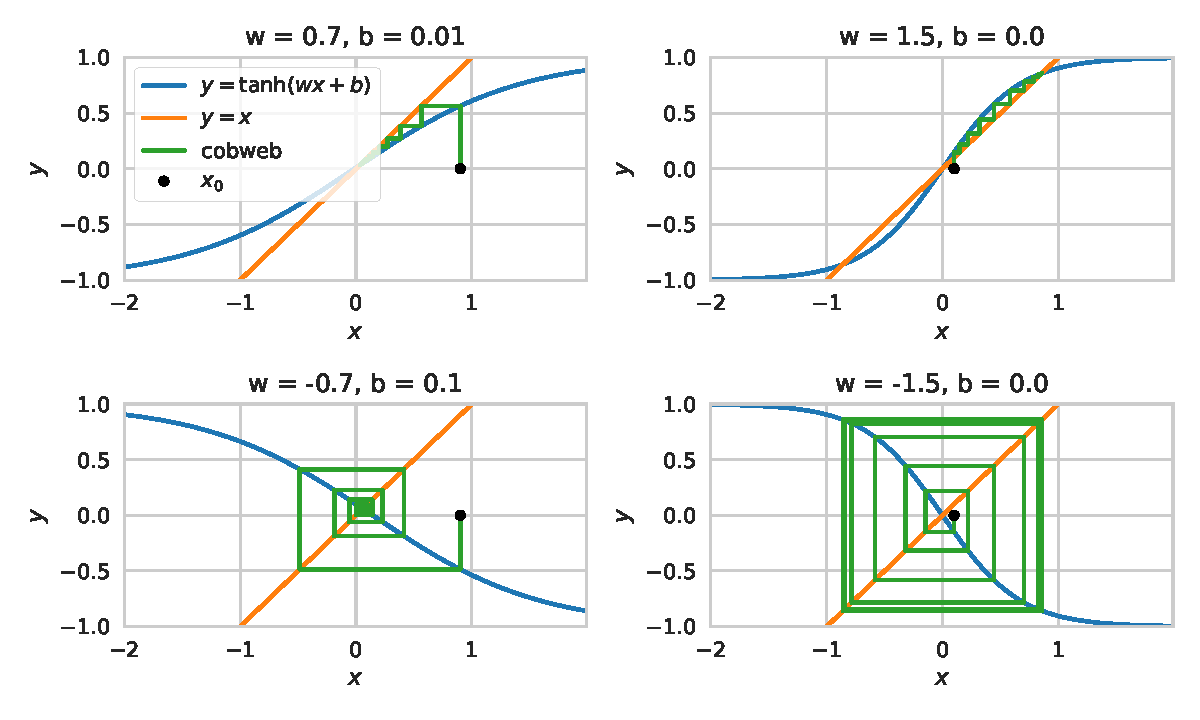
\includegraphics[width=\linewidth]{cobweb.pdf}
  \caption{Cobwebs for the same parameters as in Fig.~\ref{fig:bif_evolution}.
    The black dot is the initial value $x_0$. By drawing a vertical line to the
    intersection with the activation function gives the new input $x_1$. Drawing
    a horizontal line to the intersection with $y = x$ projects the point back to
    the $x$-axis.  The projection is the next input to the activation function.
    This process is repeated until a stable orbit or a fixed point is reached.}
  \label{fig:cobweb}
\end{figure}



By varying the parameters $w$ and $b$ the location and the nature of fixed
points can be changed. The blue line in the right plot of
Fig.~\ref{fig:fixed_points} splits in two as $w$ is increased. The point at
$w=1$ is called a \emph{bifurcation} point.  There are two things that are
happening here: the stable fixed point at $x=0$ becomes unstable (indicated by
the dashed line) and two new stable fixed points above and below zero are
created.

Fixed points can be found analytically by rewriting
Eq.~\ref{eq:single_unit_rnn} with the assumption that $x^*$ is a fixed point
(for which $x_t = x_{t+1}$):
\begin{equation}
  \label{eq:fp}
  x^* = \tanh(wx^* +b).
\end{equation}
Solving once for $w$ and once for $b$ results in two equations for fixed
points:
\begin{align}
  b &= \tanh^{-1}(x^*) - wx^*\\
  w &= \frac{\tanh^{-1}(x^*) - b}{x^*},
\end{align}
which can be plotted for different values of $w$ and $b$
(Fig.~\ref{fig:fixed_points}).  The period-2 cycles cannot be found by
analysing Eq.~\ref{eq:fp}.  Instead they can be found analytically by solving
\begin{equation}
  x^* = \tanh^2(wx^* + b),
\end{equation}
but also by an intuitive, graphical approach called \emph{cobwebbing}
(Fig.~\ref{fig:cobweb}).
Starting from an initial point $x_0$ a vertical line is drawn to the value of
the activation function. Now drawing a horizontal line until we intersect with
the graph of $y = x$ gives the new input $x_1$ and so forth.

\subsubsection{Effect on RNN Training}%
\label{ssub:effect_on_rnn_training}

Now that we have an understanding of what fixed points and bifurcations are we
can examine their effect on RNN learning. Suppose we initialize the network
with a constant $b=0.1$ and a $w=3$. If $x_0$ is negative, the nearest fixed
point is on the lower branch of the yellow line in the right plot of
Fig.~\ref{fig:fixed_points}.  Further assume we train the network to output
$x_\infty = - 0.25$.  In this case, $w$ will be lowered to approach $x^*= -
0.25$ until the bifurcation point is reached and the stable fixed point
vanishes (yellow line becomes dashed line). The fixed point becomes unstable
and the network output will change discontinuously as it jumps to the attractor
on the upper branch.  This will result in a discontinuity in the loss function
and an infinite gradient.  After jumping to the upper branch $w$ will grow
towards infinite values as the GD algorithm tries to approach the target value
of $x = - 0.25$.  Similar examples can be constructed in which parameters
oscillate between two bifurcation points.

The weights of RNNs that are used in practice are normally initialized to very
small values which results
in few fixed points. As the network learns some of the weights increase which
drives the RNN through bifurcations.  The discontinuities that result in very
large gradients cause large jumps of the GD algorithm which can nullify the
learning of hundreds of steps in a single iteration. Aside from the vanishing
and exploding gradient problems, bifurcations are another major reason for the
intricacy of RNN training.

\begin{figure}
  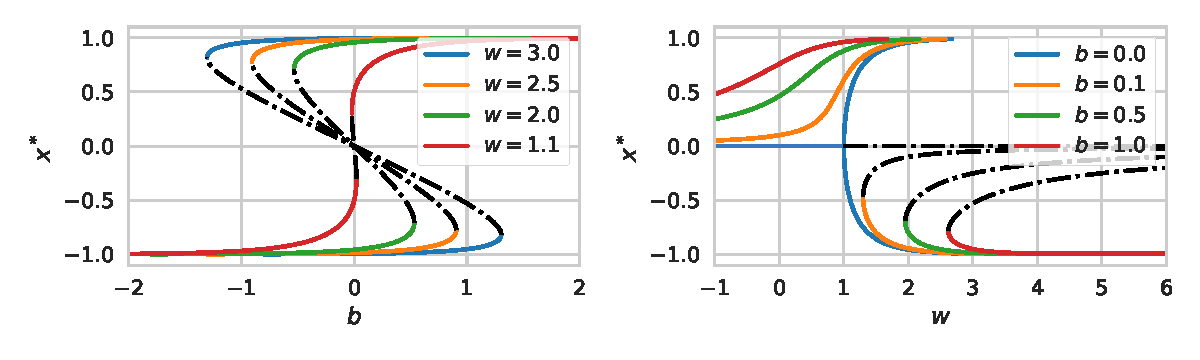
\includegraphics[width=\linewidth]{bif_fixpoints.pdf}
  \caption{Fixed points for different parameter values of $b$ and $w$.  The
    values of the fixed points $x^*$ are affected by varying the weights of the
    RNN.  If there is more than one stable fixed point $x_t$ converges to the
    attractor that is closest to the initial value $x_0$.  Dashed lines denote
    unstable fixed points, which can only be reached if $x_0 = x^*$.}
  \label{fig:fixed_points}
\end{figure}

One solution to all the headaches that are caused by the bifurcations in the
state space, and RNN training in general, is surprisingly simple.  The cause of
bifurcations are adaptions of the recurrent weights of the RNN, so keeping them
constant would eliminate all the complications at once and even come with the
additional advantage of not having to change those weights in the first place.
This might seem like a rather drastic method as the whole ML approach is based on
gradual learning of weights. However, restricting the weight optimization to the
non-recurrent weights frees us from the notorious problems of RNNs and can
perform just as well.  This approach is called \emph{reservoir computing} and
will be discussed in the next Section.
